\scanpage{105}
grâce au

\uline{Lemme}\quad a) Soit $\unsure{E|F}$ (loc.) constructible dans $X$, \inserted{($E$ loc. const.)} alors $F\cap E$ est (loc) constructible dans $E$

b) Soit $F\subset E$, \inserted{avec $E$ (loc) constructible} alors $F$ est (loc.) const. dans $E$ ssi il l'est dans $X$.

\margin{\figure{\begin{tikzpicture}\draw (0,0)--(0,-0.5);\draw (0.1,-1.1)--(0.15,-1.55);\end{tikzpicture}}}

Dém. Pour a), on montre que si $F$ est ouvert rétrocompact dans $X$, alors $F\cap E$ est rétrocompact dans $E$, grâce au fait que \unsure{$\forall$} ouvert quasi cpt $U$ de $E$ est induit par un ouvert $V$ de $X$, qu'on peut \unsure{si on veut} [grâce à l'hyp préliminaire de la prop] supposer quasi cpt, d'où
\[
f^{-1}(F)\cap U=f^{-1}(F\cap V)=\text{image inverse}
\]
d'un quasi cpt, qui est quasi cpt car $E$ est rétrocompact dans $X$, \inserted{par $\unsure{0_{\mathrm{III}}}$ 9.1.13.} \deleted{Donc} Le cas ``localement'' en résulte aussitôt, utilisant le fait que $E$ induit un $E\cap U$ constructible dans \deleted{\unsure{tt}} $U$ ouvert.

\margin{\diagram{\begin{tikzcd}[ampersand replacement=\&,column sep=small,row sep=small]
E\arrow[d,"f"']\& f^{-1}(F)\cap U\\
X\&F
\end{tikzcd}}}

Pour b), on suppose $F\subset E$ constructible dans \uline{$E$}, \inserted{construct.} prouvons que $F$ l'est dans $X$. On peut supposer $F$ \deleted{\unsure{ouvert}}\inserted{\deleted{fermé}\inserted{ouvert}} dans $E$, rétrocompact dans $E$, \deleted{et}\inserted{\unsure{puis: on}} $E=U\cap\complement V$, $U$ et $V$ rétrocomp. dans $X$ \inserted{\unsure{qui sont constructibles}}

[car $E=\bigcup E_i$ réunion finie de tels, les \deleted{$F\cap E_i$ est} dans \uline{$E$} par a), donc $E_i\cap F$ const. dans $E_i$ par a), et on est ramené à prouver qu'ils sont constructibles dans $X$, puisque $F=\bigcup E_i\cap F$.

\margin{$\unsure{0_{\mathrm{III}}}$ 9.1.8 \unsure{(i)(ii)}}

\inserted{Remplaçant $X$ par $U$, on peut supposer $E$}
\deleted{On suppose $F$ est \unsure{ouvert} dans $E$, \illegible{2}}
\inserted{\unsure{se borne au cas} $X=U$}
\deleted{$F=E\cap W$, $W$ \unsure{ouvert} dans $X$, \illegible{2}}
\margin{[$E$ étant const. dans $U$, $F$ \inserted{(par ii)} \unsure{le sera} dans $U$, donc dans $X$]}

\figure{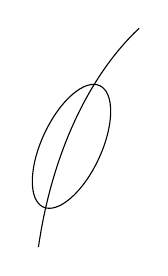
\begin{tikzpicture}[x=1cm,y=1cm]
\draw[rotate=-25] (0,0) ellipse (0.38cm and 0.85cm);
\draw (-0.42,-1.28)..controls(-0.25,-0.1)and(0.22,0.9)..(0.86,1.5);
\end{tikzpicture}}
\margin{104}
